\opred
 $\lim\limits_{x\rightarrow 0} \frac{\sin(x)}{x}=1$

\subsubsection{Доказательство}
\begin{wrapfigure}{r}[5pt]{0.4\textwidth}
	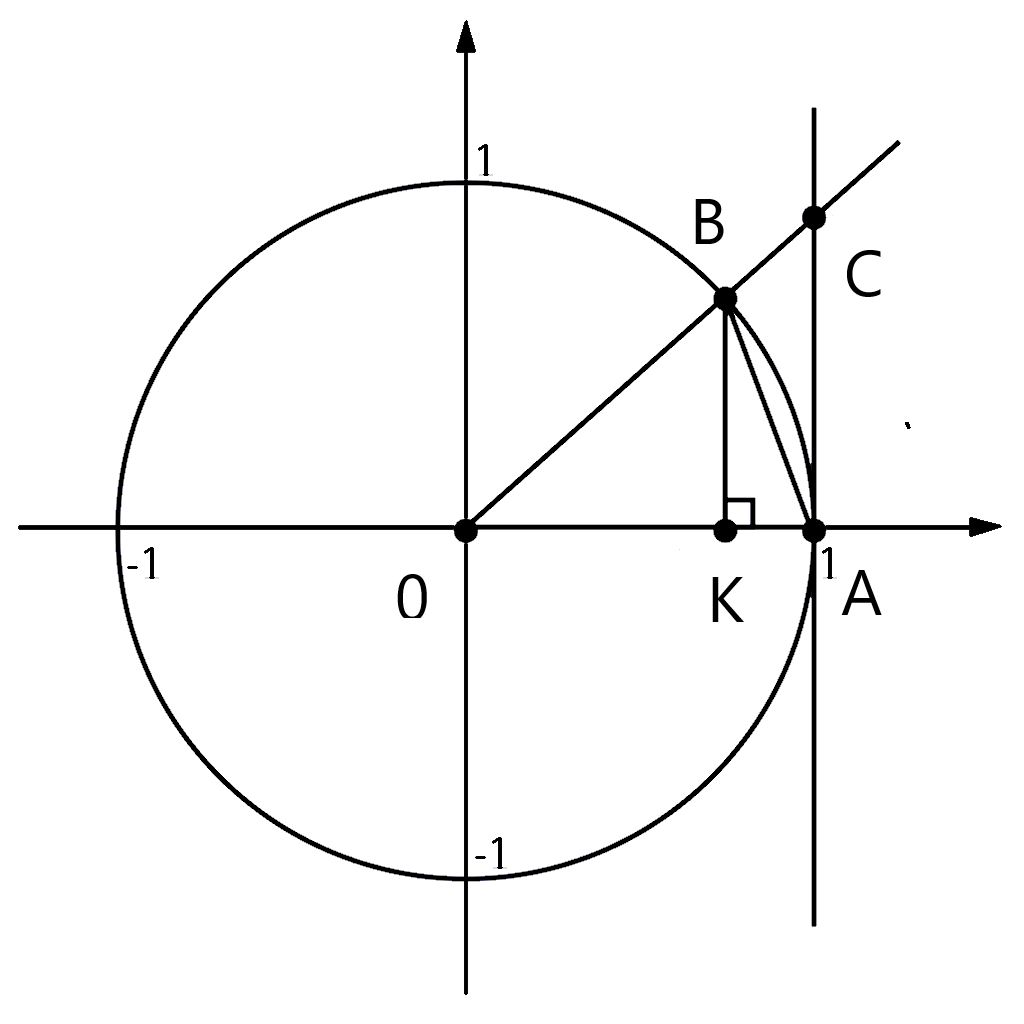
\includegraphics[scale=0.2]{image.png}
\end{wrapfigure}

Рассмотрим $\triangle$ DAB, $\triangle$ DAC и сектор OAB.
x-длинна дуги.
При $x \rightarrow 0$ их S уменьшаются.


$$ S\triangle{OBA} = \frac{1}{2}OA \cdot BK = \frac{\sin(x)}{2}$$
$$ S\triangle{OCA} = \frac{1}{2}OA \cdot AC = \frac{\operatorname{tg}(x)}{2}$$
$$ S(OBA) = \frac{1}{2}x \cdot r = \frac{x}{2}.$$

т.к. $ S\triangle OBA < SOBA < SOCA$
$\sin(x) < x < \operatorname{tg}(x)$

  $1  < \frac{x}{\sin(x)} < \frac{1}{\cos(x)}$

  $1 > \frac{\sin(x)}{x} > \cos(x)$

  это неравенство верно $\forall (x: 0 < |x|<\frac{\pi}{2})$.

  Функция, предел которой надо найти лежит между двумя функциями:
   $$\forall(\epsilon>0)\exists(\beta>0)\forall(x \in \mathbb{R})[0 < |x| <\beta \Rightarrow |\cos(x) - 1| < \epsilon]$$
  $$|\cos(x) - 1| = |2\sin^2(\frac{X}{2})| \leq 2|\sin\frac{x}{2}| < \frac{2|x|}{2} = |x| < \epsilon.$$

  Мы нашли $\beta : \beta = \epsilon$, т.к. |x| < $\beta$ и |x| < $\epsilon$. Получается:
  $$\lim\limits_{x\rightarrow 0}1=1, \lim\limits_{x \rightarrow 0}\cos(x) = 1
  \Rightarrow \lim\limits_{x \rightarrow 0}\frac{\sin(x)}{x}=1.$$
